%% —------------------------------------------------------------ %%
%% sbcreviews-2025.cls
%% Template para SBC Reviews 
%% (https://journals-sol.sbc.org.br/index.php/reviews/) 
%% 
%% Esta versão do template para a SBC Reviews inclui algumas
%% modificações sobre o template original da REIC
%% (https://journals-sol.sbc.org.br/index.php/reic)
%%
%% Licença CC BY 4.0 (https://creativecommons.org/licenses/by/4.0/)
%% Sociedade Brasileira de Computação.

\documentclass[portuguese]{sbcreviews-2025}%

%\usepackage{graphicx}% já está incluido na classe
%\usepackage[utf8]{inputenc} % obsoleto, desnecessário

\usepackage[misc,geometry]{ifsym} 

%%%%  %\usepackage{fontspec}

%% Os problemas com a classe eram originados por carregarem ambos os
%% pacotes fontenc e fontspec simultaneamente. Agora a classe detecta
%% qual engine está em uso e se for o pdflates então carrega o
%% fontenc. Se forem o xelatex ou lualatex então carrega o
%% fontspec. Eu particularemnte prefiro o lualatex ou o xetex


% \usepackage{fontawesome} %%% incluido na classe. Desnecessário
% chamá-lo aqui

%%%% \usepackage{academicons}
%%%% outro encrenqueiro que se tornou desnecessario. Deste typeface só
%%%% se usava o glifo do orcid e o codigo interno bombava.
%%%% Substitui pelo pacote orcidlink (carregado internamete na classe)
%%%% e consertei o codigo na classe.

%\usepackage{color} % carregada dentro da classe
%\usepackage{hyperref} % carregada dentro da classe

\usepackage{aas_macros}
\usepackage[bottom]{footmisc}

%\usepackage{supertabular}
%\usepackage{multicol}
%\usepackage{multirow}
%% O pacote tabularray é muito melhor para
% a criacao de tabela complexas e/ou loooongas; tudo de modo simples.
%% Torna o uso de multicol e multirow desnecessarios

\usepackage{tabularray}

\usepackage{afterpage}
\usepackage{url}
\usepackage{pifont}

\setcitestyle{square}

\definecolor{engtitle}{rgb}{0.5,0.5,0.5}
\definecolor{orcidlogo}{rgb}{0.37,0.48,0.13}
\definecolor{unilogo}{rgb}{0.16, 0.26, 0.58}
\definecolor{maillogo}{rgb}{0.58, 0.16, 0.26}
\definecolor{darkblue}{rgb}{0.0,0.0,0.0}
\hypersetup{colorlinks,breaklinks,
            linkcolor=darkblue,urlcolor=darkblue,
            anchorcolor=darkblue,citecolor=darkblue}
%\hypersetup{colorlinks,citecolor=blue,linkcolor=blue,urlcolor=blue}

%%%%%%% IMPORTANT: We disable hyperlinks by default with this line, to avoid the error "\pdfendlink ended up in different nesting level" while writing.
%\hypersetup{draft}

\jid{ROCS}
\jtitle{SBC Computing Reviews, 202X, XX:1}
\issn{2966-3938}
\doi{10.5753/rocs.202X.XXXXXX}
\copyrightstatement{This work is licensed under a Creative Commons Attribution 4.0 International License}
\jyear{202X}

\category{Revisão da Literatura}
\title[Template da SBC Reviews 2025 para artigos em português]{Apresentação do template da SBC Reviews 2025 - Versão para artigos em português}
\engtitle{\textcolor{engtitle}{Presenting the SBC Reviews 2025 template - Version for papers in Portuguese}}


%THE ORCID IS MANDATORY FOR EACH AUTHOR IN ROCS
\author[Silva et al. 202X]{
\affil{\textbf{João Silva}~\orcidlink{0000-0000-0000-0000}~\textcolor{blue}{\faEnvelope}~~[{Universidade Federal}~|\href{mailto: ...}{~{\textit{...@...br}}}~]}

\affil{\textbf{Maria Santos}~\orcidlink{0000-0000-0000-0000}~[{Universidade Federal}~|\href{mailto: ...}{~{\textit{...@...br}}}~]}

\affil{\textbf{Ana Silva }~\orcidlink{0000-0000-0000-0000}~[{Universidade Federal}~|\href{mailto: ...}{~{\textit{...@...br}}}~]}

\affil{\textbf{José Santos}~\orcidlink{0000-0000-0000-0000}~[{Universidade Federal}~|\href{mailto: ...}{~{\textit{...@...br}}}~]}

}

\begin{document}

\begin{frontmatter}

\maketitle

\begin{mail}
Instituto ..., Universidade ..., Endereço, Cidade, Estado, CEP, Brasil. 
\end{mail}


\begin{abstract-pt}
Este texto, em formato de artigo científico, tem por objetivo apresentar o novo modelo para artigos da SBC, descrevendo suas principais características e explicando como deve ser utilizado. Esta versão, mais especificamente, deve ser utilizada exclusivamente para artigos escritos em português que serão publicados em alguma série de anais de eventos na SBC OpenLib. O resumo em português, como pode-se notar neste exemplo, deve vir antes do resumo em inglês (abstract) e ter entre 500 e 750 palavras.
\end{abstract-pt}

\begin{abstract-en}
This text, formatted as a scientific article, aims to present the new SBC paper template, describing its main features and explaining how it should be used. This version, more specifically, should be used exclusively for articles written in Portuguese that will be published in any event proceeding series at SBC OpenLib. The abstract in Portuguese, as you can see in this example, must be before the abstract in English and must have between 500 and 750 words.
\end{abstract-en}

\begin{pchaves}
Anais de evento, Modelo, SBC OpenLib, Indexação
\end{pchaves}

\begin{keywords}
Proceedings, Template, SBC OpenLib, Indexing
\end{keywords}

\begin{dates}
% This information will be provided by the editor before publishing the paper
\noindent{\sffamily\textbf{Recebido/Received:}} DD Month YYYY~~~$\bullet$~~~
{\sffamily\textbf{Aceito/Accepted:}} DD Month YYYY~~~$\bullet$~~~
{\sffamily\textbf{Publicado/Published:}} DD Month YYYY
\end{dates}


%\begin{license}
%Published under the Creative Commons Attribution 4.0 International Public License (CC BY 4.0)
%\end{license}

\end{frontmatter}

\section{Introdução}
\label{sec:intro}

A classe \textsl{sbc-reviews-2025} tem com base a classe \textsl{sbc2025}, projetada para trabalhar com os \textit{engines} xetex e luatex. Dessa forma, deve-se compilar o documento com esses engines.
\begin{enumerate}
    \item no Overleaf, ajustando no menu opção de compilação para \textbf{xelatex} ou \textbf{lualatex}.\footnote{Os engines são denominados xetex e luatex. Já os comandos de compilação são \textsl{xelatex} e \textsl{lualatex}.}
    \item se compilando localmente, na sua IDE faça o ajuste do compilador. Se usuário raiz, no terminal de comando, digite \textsl{xelatex filename} ou \textsl{lualatex filename}. Não é necessário digitar a extensão \textsl{tex}.
\end{enumerate}

A classe \textsl{sbc-reviews-2025} inclui internamente os pacotes xcolor, graphicx, amsmath amssymb, hyperref, babel; 
consequentemente, não há necessidade de incluí-los no preâmbulo.

Quem tentar compilar usando a opção \texttt{pdflatex} no Overleaf vai receber uma mensagem de erro solicitando o usuário a ajustar a opção de compilação.

Para a pergunta \textit{Por que não funciona com o \texttt{pdflatex}}? Pdflatex usa um esquema de codificação de fontes complexo. O fonte \texttt{academicons}\footnote{Do fonte em questão usa-se apenas o glifo associado ao Orcid.} não tem as definições necessárias para uso com o \texttt{pdflatex}. Enquanto isso não for realizado, \texttt{pdflatex} não pode ser usado.   

\section{Sobre a SBC Reviews}

Os tópicos de interesse incluem, mas não estão limitados a:

\begin{itemize}
\item Algoritmos, Combinatória e Otimização
\item Inteligência Artificial
\item Sistemas Colaborativos
\item Biologia Computacional
\item Inteligência Computacional
\item Computação Gráfica e Processamento de Imagens
\item Redes de Computadores e Sistemas Distribuídos
\item Ontologias Computacionais
\item Engenharia de Sistemas Computacionais
\item Computação Aplicada à Saúde
\item Educação em Computação
\item Modelagem Conceitual
\item Bancos de Dados
\item Projeto de Circuitos e Sistemas Integrados
\item Jogos Digitais e Entretenimento
\item Sistemas Tolerantes a Falhas
\item Métodos Formais
\item Geoinformática
\item Computação Verde
\item Arquitetura e Processamento de Computadores de Alto Desempenho
\item Aspectos Humanos e Sociais na Computação
\item Interação Humano-Computador
\item Informática na Educação
\item Segurança da Informação e de Sistemas Computacionais
\item Informação Sistemas
\item Sistemas Multimídia e Web
\item Computação Musical
\item Processamento de Linguagem Natural
\item Linguagens de Programação
\item Robótica
\item Engenharia de Software
\item Realidade Virtual
\end{itemize}

Os dois pacotes \texttt{fontenc} e \texttt{fontspec} pertencem a ``universos'' distintos e não devem ser ambos incluídos no mesmo preâmbulo sob a pena de conflitos.

O pacote \texttt{fontspec} lida com o universo dos fontes Truetype e/ou Opentype. 
A distribuição TeXlive---a qual é usada pelo Overleaf---instala uma vasta gama de fontes: por exemplo, o \textbf{TeX Gyre Termes} é o equivalente livre e gratuito do fonte \textbf{Times New Roman}. 

Obs: para os engines xetex e luatex não é obrigatório realizar a inclusão do pacote \texttt{fontspec}. A omissão faz o engine assumir valores default para fonte e suas propriedades.

Para o engine pdftex, o pacote a ser incluido deveria ser o \textbf{fontenc}. 
A inclusão desse pacote faz com que o engine leia arquivos de definição, e outros associados e com isso executa uma ligação ``estrita'' ao fonte.  

\begin{table}[!ht]
\caption{Exemplo de legenda de tabela.}
\centering
\begin{tabular}{@{}cc@{}}
\hline\hline
Dimensão & Classificação\\
\hline%
 1  & 0.6232 \\
 2  & 0.9635 \\ 
 3  & 0.9724 \\ 
 4  & 0.9690 \\ 
 5  & 0.9840 \\ 
 6  & 0.9842 \\ 
 7  & 0.9873 \\ 
 8  & 0.9884 \\
 9  & 0.9873 \\ 
 10 & 0.9898 \\ 
 11 & 0.9914 \\
\hline\hline
\end{tabular}
\label{tab1}
\end{table}

Lorem ipsum dolor sit amet, consectetur adipiscing elit, sed do eiusmod tempor incididunt ut labore et dolore magna aliqua. Ut enim ad minim veniam, quis nostrud exercitation ullamco laboris nisi ut aliquip ex ea commodo consequat. Duis aute irure dolor in reprehenderit in voluptate velit esse cillum dolore eu fugiat nulla pariatur. Excepteur sint occaecat cupidatat non proident, sunt in culpa qui officia deserunt mollit anim id est laborum (see \textbf{ Table~\ref{tab1}}). 
Assim, recomendamos fortemente o uso do pacote \texttt{tabularray}. 

\begin{table}[!ht]
\caption{Exemplo de legenda de tabela.}
\centering
\begin{tblr}{%
columns={c},
row{even}={gray9},
row{1}={bg=red!10, font=\bfseries}
}
\hline
Dimensão & Classificação\\
\hline%
 1  & 0.6 \\
 2  & 0.963 \\ 
 3  & 0.97 \\ 
 4  & 0.9690 \\ 
 5  & 0.9840 \\ 
 6  & 0.98423 \\ 
 7  & 0.9873 \\ 
 8  & 0.9884 \\
 9  & 0.9873 \\ 
 10 & 0.9898 \\ 
 11 & 0.991 \\
\end{tblr}
\label{tab1-1}
\end{table}

Lorem ipsum dolor sit amet, consectetur adipiscing elit, sed do eiusmod tempor incididunt ut labore et dolore magna aliqua. Ut enim ad minim veniam, quis nostrud exercitation ullamco laboris nisi ut aliquip ex ea commodo consequat. Duis aute irure dolor in reprehenderit in voluptate velit esse cillum dolore eu fugiat nulla pariatur. Excepteur sint occaecat cupidatat non proident, sunt in culpa qui officia deserunt mollit anim id est laborum \citep{ref3}, dolor sit amet, consectetur adipiscing elit, sed do eiusmod tempor incididunt ut labore et dolore magna aliqua. Ut enim ad minim veniam, quis nostrud exercitation ullamco laboris nisi ut aliquip ex ea commodo consequat.

Lorem ipsum dolor sit amet, consectetur adipiscing elit, sed do eiusmod tempor incididunt ut labore et dolore magna aliqua. Ut enim ad minim veniam, quis nostrud exercitation ullamco laboris nisi ut aliquip ex ea commodo consequat~\citep{ref4}.

\subsection{Modelo de Publicação}

A SBC Reviews adota o modelo de Publicação Contínua, o que significa que os artigos são publicados imediatamente após a aceitação, sem esperar pela compilação de uma edição completa. Essa abordagem acelera a disseminação e a disponibilidade de descobertas científicas, beneficiando pesquisadores, estudantes, leitores, editoras e agências de fomento, promovendo rapidez e acesso oportuno a pesquisas de alta qualidade para leitura e citação.

\subsection{Acesso Aberto Diamante}

A SBC Reviews é de acesso aberto e gratuito para autores e leitores. Todos os artigos publicados pela SBC Reviews são disponibilizados online de forma gratuita e permanente imediatamente após a publicação, sem taxas de assinatura ou barreiras de registro. Acreditamos que a política adotada elimina barreiras econômicas e geográficas, promove a democratização global e acelera o progresso da pesquisa.

\subsection{Aviso de Direitos Autorais}
Os autores que publicam na SBC Reviews mantêm os direitos autorais de seus artigos e autorizam a SBC a publicá-los sob os termos da Licença Pública Internacional Creative Commons Atribuição 4.0 (CC BY 4.0). Assim, os autores ou terceiros podem reproduzir ou distribuir, no todo ou em parte, conteúdo extraído dos artigos publicados, na íntegra, adaptado ou remixado, desde que sejam atribuídos os devidos créditos aos autores originais e à publicação original.

\section{Submissões}

\subsection{Checklist de Preparação para Submissão}

Como parte do processo de submissão, os autores devem verificar a conformidade de sua submissão com todos os itens a seguir. As submissões poderão ser devolvidas aos autores que não seguirem estas diretrizes.

\section{Revisões de Literatura}

Revisões de literatura são estudos retrospectivos e observacionais.
A SBC Reviews publica revisões de literatura em áreas de pesquisa em Computação, incluindo, entre outros, os seguintes tipos de revisão:

\textbf{Revisões sistemáticas de literatura} são revisões rigorosas e abrangentes que visam responder a uma questão de pesquisa específica e focada, avaliando e sintetizando criticamente todos os estudos de pesquisa originais relevantes. Se métodos estatísticos forem usados para combinar dados quantitativos de vários estudos, trata-se de um estudo de Meta-Análise.

\textbf{Revisões multivocais da literatura} são um tipo de RSL que incorpora tanto literatura formal revisada por pares (como artigos de periódicos e trabalhos de conferências) quanto literatura cinzenta. A literatura cinzenta inclui materiais como relatórios técnicos, postagens em blogs e apresentações em conferências, que podem não ser formalmente publicados ou revisados por pares.

\textbf{Revisões de escopo} abordam questões de pesquisa mais amplas e exploratórias para mapear a extensão, o alcance e a natureza da pesquisa sobre um tópico específico. Entre outros objetivos, as revisões de escopo ajudam a determinar se uma revisão sistemática da literatura é necessária.

\textbf{Mapeamentos sistemáticos da literatura} concentram-se na categorização e quantificação da literatura existente para fornecer uma visão geral da atividade de pesquisa em um subcampo.

O periódico SBC Reviews também avalia submissões de revisões de literatura que abordam avaliações de progresso e/ou avaliações críticas relevantes para subcampos específicos.

\section{Exemplo de Título Nível 1 (Seção)}
Lorem ipsum dolor sit amet, consectetur adipiscing elit, sed do eiusmod tempor incididunt ut labore et dolore magna aliqua. Ut enim ad minim veniam, quis nostrud exercitation ullamco laboris nisi ut aliquip ex ea commodo consequat. Duis aute irure dolor in reprehenderit in voluptate velit esse cillum dolore eu fugiat nulla pariatur. Excepteur sint occaecat cupidatat non proident, sunt in culpa qui officia deserunt mollit anim id est laborum. Lorem ipsum dolor sit amet, consectetur adipiscing elit, sed do eiusmod tempor incididunt ut labore et dolore magna aliqua. Ut enim ad minim veniam, quis nostrud exercitation ullamco laboris nisi ut aliquip ex ea commodo consequat. Duis aute irure dolor in reprehenderit in voluptate velit esse cillum dolore eu fugiat nulla pariatur. Excepteur sint occaecat cupidatat non proident, sunt in culpa qui officia deserunt mollit anim id est laborum.

\subsection{Exemplo de Título Nível 2 (Subseção)}

Lorem ipsum dolor sit amet, consectetur adipiscing elit, sed do eiusmod tempor incididunt ut labore et dolore magna aliqua. Ut enim ad minim veniam, quis nostrud exercitation ullamco laboris nisi ut aliquip ex ea commodo consequat. Duis aute irure dolor in reprehenderit in voluptate velit esse cillum dolore eu fugiat nulla pariatur. Excepteur sint occaecat cupidatat non proident, sunt in culpa qui officia deserunt mollit anim id est laborum.

\begin{quotation}
\textit{This is a longer quotation. Lorem ipsum dolor sit amet, consectetur adipiscing elit, sed do eiusmod tempor incididunt ut labore et dolore magna aliqua. Lorem ipsum dolor sit amet, consectetur adipiscing elit, sed do eiusmod tempor incididunt ut labore et magna aliqua. 
}\end{quotation} 

\subsubsection{Exemplo de Título Nível 3 (Subsubseção)}

Lorem ipsum dolor sit amet, consectetur adipiscing elit, sed do eiusmod tempor incididunt ut labore et dolore magna aliqua. Ut enim ad minim veniam, quis nostrud exercitation ullamco laboris nisi ut aliquip ex ea commodo consequat. Duis aute irure dolor in reprehenderit in voluptate velit esse cillum dolore eu fugiat nulla pariatur. Excepteur sint occaecat cupidatat non proident, sunt in culpa qui officia deserunt mollit anim id est laborum. Lorem ipsum dolor sit amet, consectetur adipiscing elit, sed do eiusmod tempor incididunt ut labore et dolore magna aliqua. Ut enim ad minim veniam, quis nostrud exercitation ullamco laboris nisi ut aliquip ex ea commodo consequat. Duis aute irure dolor in reprehenderit in voluptate velit esse cillum dolore eu fugiat nulla pariatur. Excepteur sint occaecat cupidatat non proident, sunt in culpa qui officia deserunt mollit anim id est laborum.

\paragraph{Exemplo de Título Nível 4 (Parágrafo).}

Lorem ipsum dolor sit amet, consectetur adipiscing elit, sed do eiusmod tempor incididunt ut labore et dolore magna aliqua. Ut enim ad minim veniam, quis nostrud exercitation ullamco laboris nisi ut aliquip ex ea commodo consequat. Duis aute irure dolor in reprehenderit in voluptate velit esse cillum dolore eu fugiat nulla pariatur. Excepteur sint occaecat cupidatat non proident, sunt in culpa qui officia deserunt mollit anim id est laborum. 
Let
\[
x=(x_1,\dots,x_n)\in R^n
\]be an \(n\)-dimensional vector. The sparse PCA problem can be written as
\begin{equation}\label{eq1}
\max\limits_{x}\{x^TAx-\rho\|x\|_0:x^Tx=1\},
\end{equation}
Lorem ipsum dolor sit amet, consectetur adipiscing elit, sed do eiusmod tempor incididunt ut labore et dolore magna aliqua. Ut enim ad minim veniam, quis nostrud exercitation ullamco laboris nisi ut aliquip ex ea commodo consequat. Duis aute irure dolor in reprehenderit in voluptate velit esse cillum dolore eu fugiat nulla pariatur\break equation (\ref{eq1}). 
\[\max\limits_{x}\{x^TAx :x^Tx=1\}.\]
If $A$ Lorem ipsum dolor sit amet, consectetur adipiscing elit, sed do eiusmod tempor incididunt ut labore et dolore magna aliqua. Ut enim ad minim veniam, quis nostrud exercitation ullamco laboris nisi ut aliquip ex ea commodo consequat. 


Equation (\ref{eq1}) is a special case of the following sparse generalized eigenvector problem (GEV):
\begin{equation}\label{GEV}
\max\limits_{x}\{x^TAx-\rho \|x\|_0: x^TBx\leq 1\},
\end{equation}

Lorem ipsum dolor sit amet, consectetur adipiscing elit, sed do eiusmod tempor incididunt ut labore et dolore magna aliqua. Ut enim ad minim veniam, quis nostrud exercitation ullamco laboris nisi ut aliquip ex ea commodo consequat. Duis aute irure dolor in reprehenderit in voluptate velit esse cillum dolore eu fugiat nulla pariatur. Excepteur sint occaecat cupidatat non proident, sunt in culpa qui officia deserunt mollit anim id est laborum. 

Lorem ipsum dolor sit amet, consectetur adipiscing elit, sed do eiusmod tempor incididunt ut labore et dolore magna aliqua. Ut enim ad minim veniam, quis nostrud exercitation ullamco laboris nisi ut aliquip ex ea commodo consequat. Duis aute irure dolor in reprehenderit in voluptate velit esse cillum dolore eu fugiat nulla pariatur. Excepteur sint occaecat cupidatat non proident, sunt in culpa qui officia deserunt mollit anim id est laborum \textbf{Table~\ref{tab2}}.

\section{Exemplo de Título Nível 1}

Lorem ipsum dolor sit amet, consectetur adipiscing elit, sed do eiusmod tempor incididunt ut labore et dolore magna aliqua. Ut enim ad minim veniam, quis nostrud exercitation ullamco laboris nisi ut aliquip ex ea commodo consequat. Duis aute irure dolor in reprehenderit in voluptate velit esse cillum dolore eu fugiat nulla pariatur. Excepteur sint occaecat cupidatat non proident, sunt in culpa qui officia deserunt mollit anim id est laborum. Lorem ipsum dolor sit amet, consectetur adipiscing elit, sed do eiusmod tempor incididunt ut labore et dolore magna aliqua. Ut enim ad minim veniam, quis nostrud exercitation ullamco laboris nisi ut aliquip ex ea commodo consequat. Duis aute irure dolor in reprehenderit in voluptate velit esse cillum dolore eu fugiat nulla pariatur. Excepteur sint occaecat cupidatat non proident, sunt in culpa qui officia deserunt mollit anim id est laborum.


\begin{table*}
\caption{Exemplo de legenda de tabela.  Duis aute irure dolor in reprehenderit in voluptate velit esse cillum dolore eu fugiat nulla pariatur. Excepteur sint occaecat cupidatat non proident, sunt in culpa qui officia deserunt mollit.} 
\centering
\begin{tabular*}{\textwidth}{@{}c\x c\x c\x c\x c\x c\x c\x c\x c\x c\x c\x c@{}}
\hline \hline
 Número   &  Vel (km/h)   & $\alpha$ (m/s$^2$)    &  $\epsilon^{(1)}$  &  $\epsilon^{(2)}$ 
         & $\delta^{(1)}$ & $\delta^{(2)}$  &  $\delta^{(3)}$    & $\gamma^{(1)}$ 
         & $\gamma^{(2)}$ & $\alpha^{(1)}$  & $\alpha^{(2)}$ \\
%
\hline
 1 & 3.5 & 2.0 & 0.20 & -0.05 & 0.00 & -0.20 & -0.05 & 0.20 & ~0.05 & 20 & 10 \\ 
 2 & 2.5 & 1.5 & 0.10 & -0.15 & 0.05 & -0.15 & ~0.00 & 0.10 & -0.05 & 20 & 40 \\ 
 3 & 3.0 & 1.8 & 0.20 & -0.05 & 0.25 & ~0.05 & ~0.20 & 0.15 & ~0.00 & 20 & 70$^a$ \\
\hline \hline
\end{tabular*}\label{tab2}
\end{table*}

Lorem ipsum dolor sit amet, consectetur adipiscing elit, sed do eiusmod tempor incididunt ut labore et dolore magna aliqua. Ut enim ad minim veniam, quis nostrud exercitation ullamco laboris nisi ut aliquip ex ea commodo consequat. Duis aute irure dolor in reprehenderit in voluptate velit esse cillum dolore eu fugiat nulla pariatur. Excepteur sint occaecat cupidatat non proident, sunt in culpa qui officia deserunt mollit anim id est laborum. Lorem ipsum dolor sit amet, consectetur adipiscing elit, sed do eiusmod tempor incididunt ut labore et dolore magna aliqua. Ut enim ad minim veniam, quis nostrud exercitation ullamco laboris nisi ut aliquip ex ea commodo consequat. Duis aute irure dolor in reprehenderit in voluptate velit esse cillum dolore eu fugiat nulla pariatur. Excepteur sint occaecat cupidatat non proident, sunt in culpa qui officia deserunt mollit anim id est laborum.

\begin{itemize}
\item Esse é um exemplo de lista de tópicos. Lorem ipsum dolor sit amet, consectetur adipiscing elit, sed do eiusmod tempor incididunt.
\item Lorem ipsum dolor sit amet, consectetur adipiscing elit, sed do eiusmod tempor incididunt ut labore et dolore magna aliqua. Ut enim ad minim veniam.
\item Lorem ipsum dolor sit amet, consectetur adipiscing elit, sed do eiusmod tempor incididunt ut labore et dolore magna aliqua. Ut enim ad minim veniam.
\end{itemize}

Lorem ipsum dolor sit amet, consectetur adipiscing elit, sed do eiusmod tempor incididunt ut labore et dolore magna aliqua. Ut enim ad minim veniam, quis nostrud exercitation ullamco laboris nisi ut aliquip ex ea commodo consequat. Duis aute irure dolor in reprehenderit in voluptate velit esse cillum dolore eu fugiat nulla pariatur. Excepteur sint occaecat cupidatat non proident, sunt in culpa qui officia deserunt mollit anim id est laborum. Lorem ipsum dolor sit amet, consectetur adipiscing elit, sed do eiusmod tempor incididunt ut labore et dolore magna aliqua. Ut enim ad minim veniam, quis nostrud exercitation ullamco laboris nisi ut aliquip ex ea commodo consequat. Duis aute irure dolor in reprehenderit in voluptate velit esse cillum dolore eu fugiat nulla pariatur. Excepteur sint occaecat cupidatat non proident, sunt in culpa qui officia deserunt mollit anim id est laborum.

\begin{enumerate}%
\item Esse é um exemplo de lista numerada. Lorem ipsum dolor sit amet, consectetur adipiscing elit, sed do eiusmod tempor incididunt.
\item Lorem ipsum dolor sit amet, consectetur adipiscing elit, sed do eiusmod tempor incididunt ut labore et dolore magna aliqua. Ut enim ad minim veniam.
\item Lorem ipsum dolor sit amet, consectetur adipiscing elit, sed do eiusmod tempor incididunt ut labore et dolore magna aliqua. Ut enim ad minim veniam.
\end{enumerate}

Lorem ipsum dolor sit amet, consectetur adipiscing elit, sed do eiusmod tempor incididunt ut labore et dolore magna aliqua. Ut enim ad minim veniam, quis nostrud exercitation ullamco laboris nisi ut aliquip ex ea commodo consequat. Duis aute irure dolor in reprehenderit in voluptate velit esse cillum dolore eu fugiat nulla pariatur. Excepteur sint occaecat cupidatat non proident, sunt in culpa qui officia deserunt mollit anim id est laborum. Lorem ipsum dolor sit amet, consectetur adipiscing elit, sed do eiusmod tempor incididunt ut labore et dolore magna aliqua. Ut enim ad minim veniam, quis nostrud exercitation ullamco laboris nisi ut aliquip ex ea commodo consequat. Duis aute irure dolor in reprehenderit in voluptate velit esse cillum dolore eu fugiat nulla pariatur. Excepteur sint occaecat cupidatat non proident, sunt in culpa qui officia deserunt mollit anim id est laborum.

Lorem ipsum dolor sit amet, consectetur adipiscing elit, sed do eiusmod tempor incididunt ut labore et dolore magna aliqua. Ut enim ad minim veniam, quis nostrud exercitation ullamco laboris nisi ut aliquip ex ea commodo consequat. Duis aute irure dolor in reprehenderit in voluptate velit esse cillum dolore eu fugiat nulla pariatur. Excepteur sint occaecat cupidatat non proident, sunt in culpa qui officia deserunt mollit anim id est laborum. Lorem ipsum dolor sit amet, consectetur adipiscing elit, sed do eiusmod tempor incididunt ut labore et dolore magna aliqua. Ut enim ad minim veniam, quis nostrud exercitation ullamco laboris nisi ut aliquip ex ea commodo consequat. Duis aute irure dolor in reprehenderit in voluptate velit esse cillum dolore eu fugiat nulla pariatur. Excepteur sint occaecat cupidatat non proident, sunt in culpa qui officia deserunt mollit anim id est laborum.


\subsection{Exemplo de Título Nível 2}

Lorem ipsum dolor sit amet, consectetur adipiscing elit, sed do eiusmod tempor incididunt ut labore et dolore magna aliqua. Ut enim ad minim veniam, quis nostrud exercitation ullamco laboris nisi ut aliquip ex ea commodo consequat. Duis aute irure dolor in reprehenderit in voluptate velit esse cillum dolore eu fugiat nulla pariatur. Excepteur sint occaecat cupidatat non proident, sunt in culpa qui officia deserunt mollit anim id est laborum. Lorem ipsum dolor sit amet, consectetur adipiscing elit, sed do eiusmod tempor incididunt ut labore et dolore magna aliqua. Ut enim ad minim veniam, quis nostrud exercitation ullamco laboris nisi ut aliquip ex ea commodo consequat. Duis aute irure dolor in reprehenderit in voluptate velit esse cillum dolore eu fugiat nulla pariatur. Excepteur sint occaecat cupidatat non proident, sunt in culpa qui officia deserunt mollit anim id est laborum \textbf{Figure \ref{Fig1}}.

Lorem ipsum dolor sit amet, consectetur adipiscing elit, sed do eiusmod tempor incididunt ut labore et dolore magna aliqua. Ut enim ad minim veniam, quis nostrud exercitation ullamco laboris nisi ut aliquip ex ea commodo consequat. Duis aute irure dolor in reprehenderit in voluptate velit esse cillum dolore eu fugiat nulla pariatur. Excepteur sint occaecat cupidatat non proident, sunt in culpa qui officia deserunt mollit anim id est laborum. Lorem ipsum dolor sit amet, consectetur adipiscing elit, sed do eiusmod tempor incididunt ut labore et dolore magna aliqua. Ut enim ad minim veniam, quis nostrud exercitation ullamco laboris nisi ut aliquip ex ea commodo consequat. Duis aute irure dolor in reprehenderit in voluptate velit esse cillum dolore eu fugiat nulla pariatur. Excepteur sint occaecat cupidatat non proident, sunt in culpa qui officia deserunt mollit anim id est laborum.

Lorem ipsum dolor sit amet, consectetur adipiscing elit, sed do eiusmod tempor incididunt ut labore et dolore magna aliqua. Ut enim ad minim veniam, quis nostrud exercitation ullamco laboris nisi ut aliquip ex ea commodo consequat. Duis aute irure dolor in reprehenderit in voluptate velit esse cillum dolore eu fugiat nulla pariatur. Excepteur sint occaecat cupidatat non proident, sunt in culpa qui officia deserunt mollit anim id est laborum. Lorem ipsum dolor sit amet, consectetur adipiscing elit, sed do eiusmod tempor incididunt ut labore et dolore magna aliqua. Ut enim ad minim veniam, quis nostrud exercitation ullamco laboris nisi ut aliquip ex ea commodo consequat. Duis aute irure dolor in reprehenderit in voluptate velit esse cillum dolore eu fugiat nulla pariatur. Excepteur sint occaecat cupidatat non proident, sunt in culpa qui officia deserunt mollit anim id est laborum.

\begin{figure}
\begin{center}
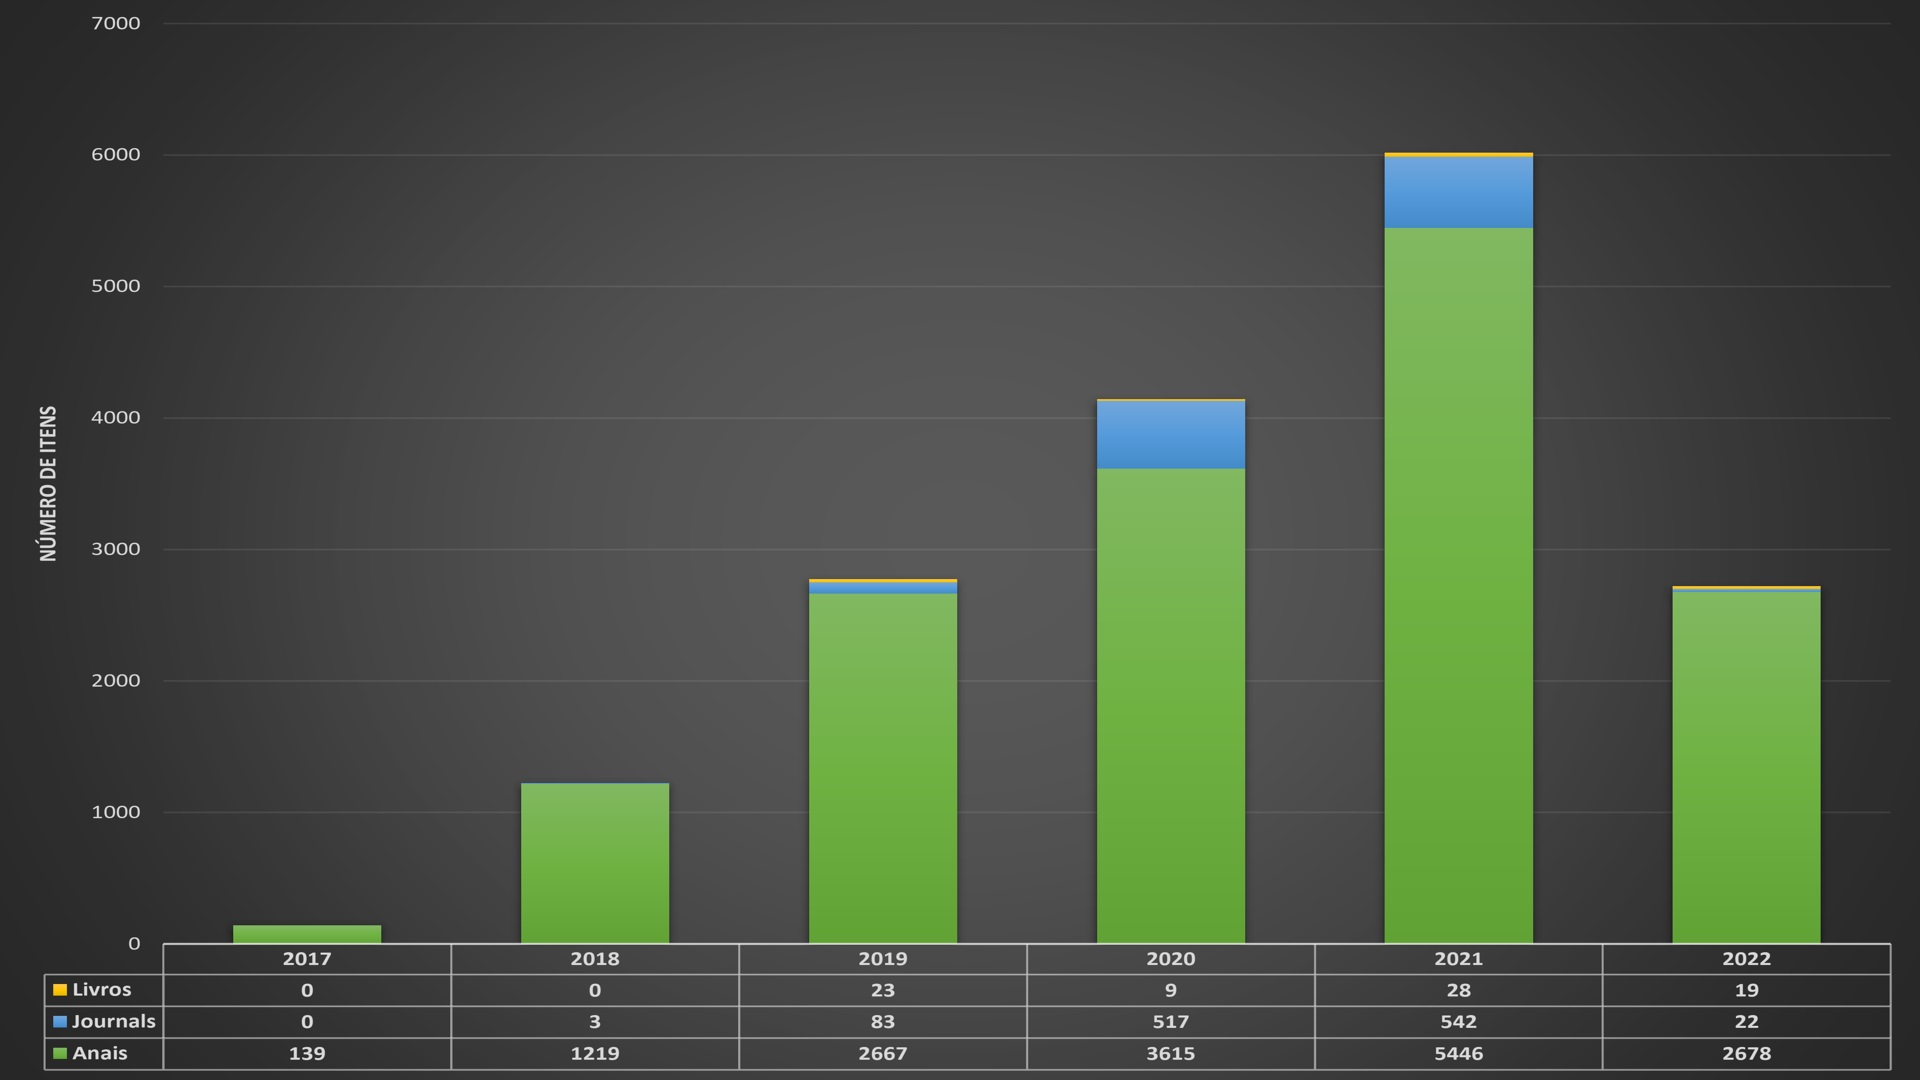
\includegraphics[width=\columnwidth]{sol.jpg}
\caption{Exemplo de legenda de figura.}\label{Fig1}
\end{center}
\end{figure}

Lorem ipsum dolor sit amet, consectetur adipiscing elit, sed do eiusmod tempor incididunt ut labore et dolore magna aliqua. Ut enim ad minim veniam, quis nostrud exercitation ullamco laboris nisi ut aliquip ex ea commodo consequat. Duis aute irure dolor in reprehenderit in voluptate velit esse cillum dolore eu fugiat nulla pariatur. Excepteur sint occaecat cupidatat non proident, sunt in culpa qui officia deserunt mollit anim id est laborum. Lorem ipsum dolor sit amet, consectetur adipiscing elit, sed do eiusmod tempor incididunt ut labore et dolore magna aliqua. Ut enim ad minim veniam, quis nostrud exercitation ullamco laboris nisi ut aliquip ex ea commodo consequat. Duis aute irure dolor in reprehenderit in voluptate velit esse cillum dolore eu fugiat nulla pariatur. Excepteur sint occaecat cupidatat non proident, sunt in culpa qui officia deserunt mollit anim id est laborum.

Lorem ipsum dolor sit amet, consectetur adipiscing elit, sed do eiusmod tempor incididunt ut labore et dolore magna aliqua. Ut enim ad minim veniam, quis nostrud exercitation ullamco laboris nisi ut aliquip ex ea commodo consequat. Duis aute irure dolor in reprehenderit in voluptate velit esse cillum dolore eu fugiat nulla pariatur. Excepteur sint occaecat cupidatat non proident, sunt in culpa qui officia deserunt mollit anim id est laborum. Lorem ipsum dolor sit amet, consectetur adipiscing elit, sed do eiusmod tempor incididunt ut labore et dolore magna aliqua. Ut enim ad minim veniam, quis nostrud exercitation ullamco laboris nisi ut aliquip ex ea commodo consequat. Duis aute irure dolor in reprehenderit in voluptate velit esse cillum dolore eu fugiat nulla pariatur. Excepteur sint occaecat cupidatat non proident, sunt in culpa qui officia deserunt mollit anim id est laborum \textbf{Figure \ref{Fig2}}.

\begin{figure*}
\begin{center}
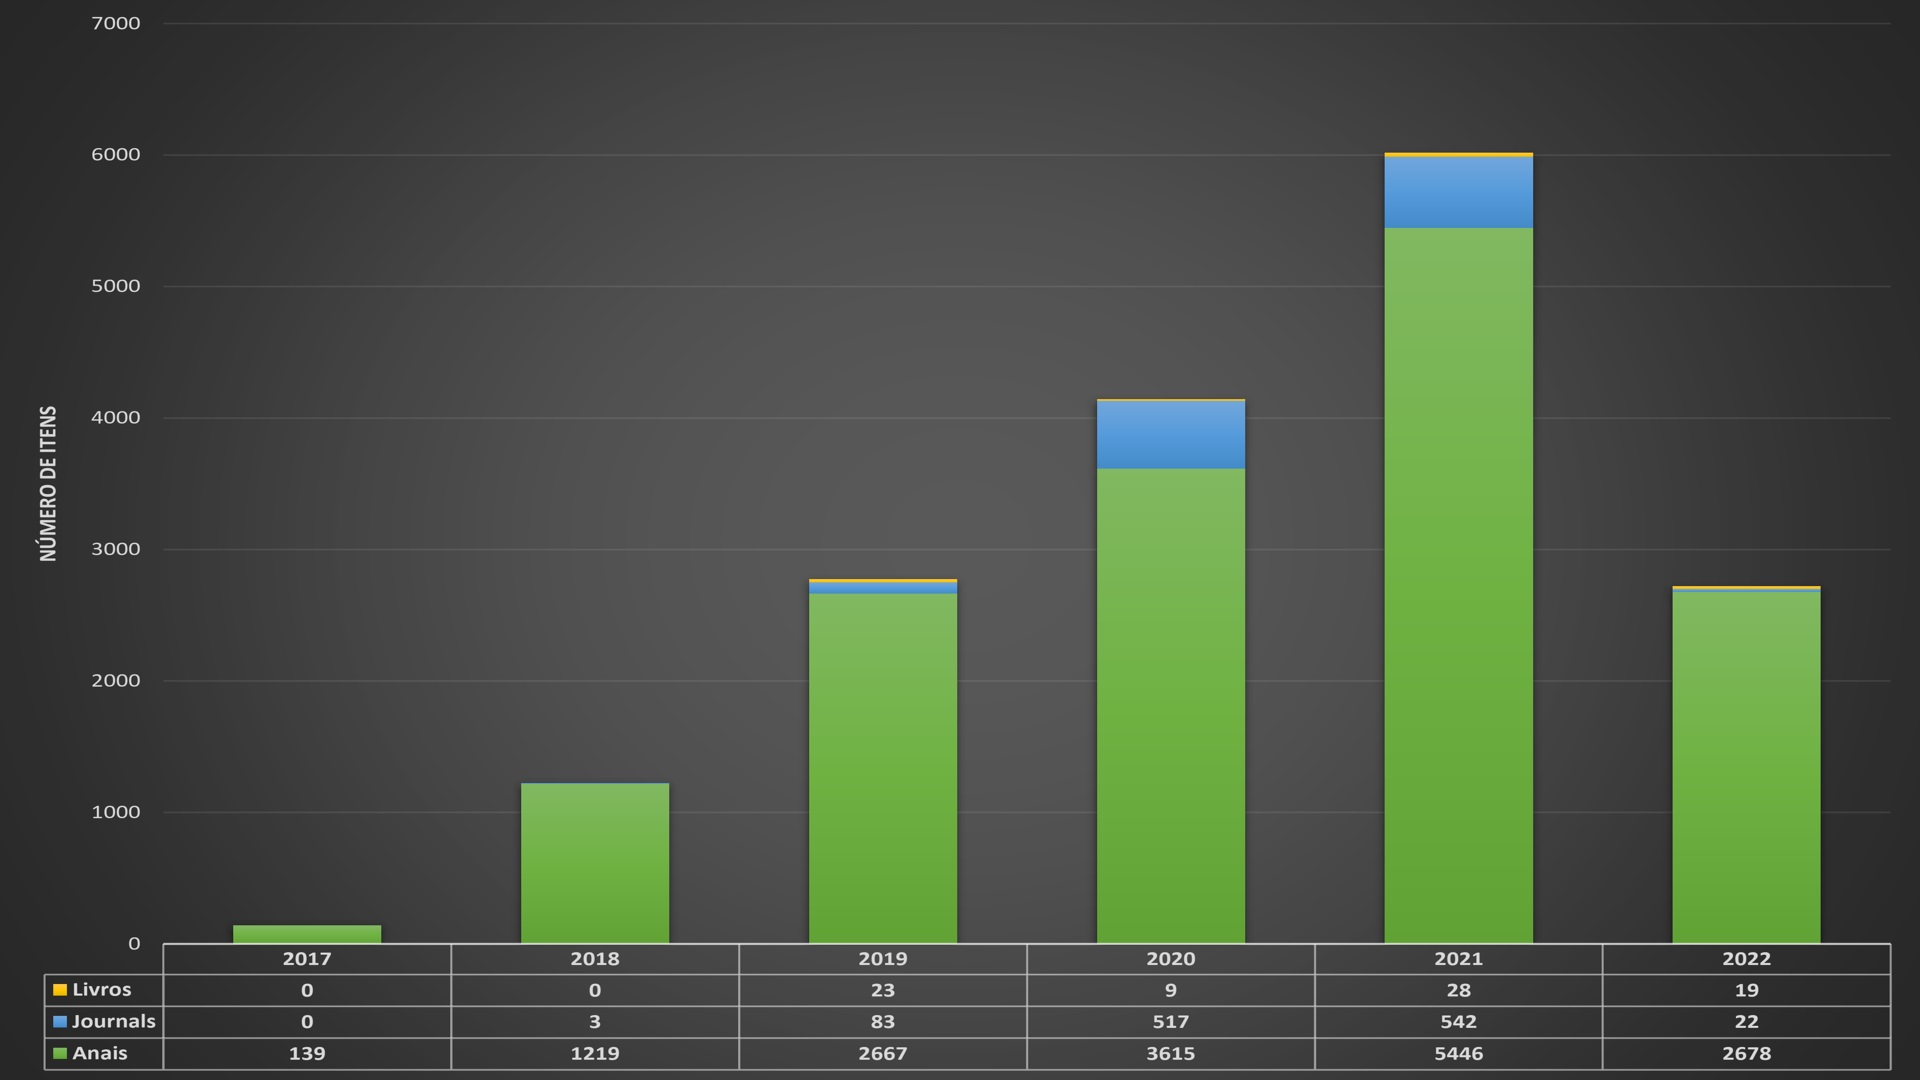
\includegraphics[width=30pc]{sol.jpg}
\caption{{Exemplo de legenda de figura.}}
 \label{Fig2}
\end{center}
\end{figure*}

Lorem ipsum dolor sit amet, consectetur adipiscing elit, sed do eiusmod tempor incididunt ut labore et dolore magna aliqua. Ut enim ad minim veniam, quis nostrud exercitation ullamco laboris nisi ut aliquip ex ea commodo consequat. Duis aute irure dolor in reprehenderit in voluptate velit esse cillum dolore eu fugiat nulla pariatur. Excepteur sint occaecat cupidatat non proident, sunt in culpa qui officia deserunt mollit anim id est laborum. Lorem ipsum dolor sit amet, consectetur adipiscing elit, sed do eiusmod tempor incididunt ut labore et dolore magna aliqua. Ut enim ad minim veniam, quis nostrud exercitation ullamco laboris nisi ut aliquip ex ea commodo consequat. Duis aute irure dolor in reprehenderit in voluptate velit esse cillum dolore eu fugiat nulla pariatur. Excepteur sint occaecat cupidatat non proident, sunt in culpa qui officia deserunt mollit anim id est laborum.

Lorem ipsum dolor sit amet, consectetur adipiscing elit, sed do eiusmod tempor incididunt ut labore et dolore magna aliqua. Ut enim ad minim veniam, quis nostrud exercitation ullamco laboris nisi ut aliquip ex ea commodo consequat. Duis aute irure dolor in reprehenderit in voluptate velit esse cillum dolore eu fugiat nulla pariatur. Excepteur sint occaecat cupidatat non proident, sunt in culpa qui officia deserunt mollit anim id est laborum. Lorem ipsum dolor sit amet, consectetur adipiscing elit, sed do eiusmod tempor incididunt ut labore et dolore magna aliqua. Ut enim ad minim veniam, quis nostrud exercitation ullamco laboris nisi ut aliquip ex ea commodo consequat. Duis aute irure dolor in reprehenderit in voluptate velit esse cillum dolore eu fugiat nulla pariatur. Excepteur sint occaecat cupidatat non proident, sunt in culpa qui officia deserunt mollit anim id est laborum.

Lorem ipsum dolor sit amet, consectetur adipiscing elit, sed do eiusmod tempor incididunt ut labore et dolore magna aliqua. Ut enim ad minim veniam, quis nostrud exercitation ullamco laboris nisi ut aliquip ex ea commodo consequat. Duis aute irure dolor in reprehenderit in voluptate velit esse cillum dolore eu fugiat nulla pariatur. Excepteur sint occaecat cupidatat non proident, sunt in culpa qui officia deserunt mollit anim id est laborum. Lorem ipsum dolor sit amet, consectetur adipiscing elit, sed do eiusmod tempor incididunt ut labore et dolore magna aliqua. Ut enim ad minim veniam, quis nostrud exercitation ullamco laboris nisi ut aliquip ex ea commodo consequat. Duis aute irure dolor in reprehenderit in voluptate velit esse cillum dolore eu fugiat nulla pariatur. Excepteur sint occaecat cupidatat non proident, sunt in culpa qui officia deserunt mollit anim id est laborum.



\paragraph{Exemplo de Título Nível 4.}

Excepteur sint occaecat cupidatat non proident, sunt in culpa qui officia deserunt mollit anim id est laborum. Lorem ipsum dolor sit amet, consectetur adipiscing elit, sed do eiusmod tempor incididunt ut labore et dolore magna aliqua. Ut enim ad minim veniam, quis nostrud exercitation ullamco laboris nisi ut aliquip ex ea commodo consequat. Duis aute irure dolor in reprehenderit in voluptate velit esse cillum dolore eu fugiat nulla pariatur. 

Lorem ipsum dolor sit amet, consectetur adipiscing elit, sed do eiusmod tempor incididunt ut labore et dolore magna aliqua. Ut enim ad minim veniam, quis nostrud exercitation ullamco laboris nisi ut aliquip ex ea commodo consequat. Excepteur sint occaecat cupidatat non proident, sunt in culpa qui officia deserunt mollit anim id est laborum. Lorem ipsum dolor sit amet, consectetur adipiscing elit, sed do eiusmod tempor incididunt ut labore et dolore magna aliqua. Ut enim ad minim veniam, quis nostrud exercitation ullamco laboris nisi ut aliquip ex ea commodo consequat. Duis aute irure dolor in reprehenderit in voluptate velit esse cillum dolore eu fugiat nulla pariatur. Excepteur sint occaecat cupidatat non proident, sunt in culpa qui officia deserunt mollit anim id est laborum.

\section{Conclusão}

Excepteur sint occaecat cupidatat non proident, sunt in culpa qui officia deserunt mollit anim id est laborum. Lorem ipsum dolor sit amet, consectetur adipiscing elit, sed do eiusmod tempor incididunt ut labore et dolore magna aliqua. Ut enim ad minim veniam, quis nostrud exercitation ullamco laboris nisi ut aliquip ex ea commodo consequat. Duis aute irure dolor in reprehenderit in voluptate velit esse cillum dolore eu fugiat nulla pariatur. 

Lorem ipsum dolor sit amet, consectetur adipiscing elit, sed do eiusmod tempor incididunt ut labore et dolore magna aliqua. Ut enim ad minim veniam, quis nostrud exercitation ullamco laboris nisi ut aliquip ex ea commodo consequat. Excepteur sint occaecat cupidatat non proident, sunt in culpa qui officia deserunt mollit anim id est laborum. Lorem ipsum dolor sit amet, consectetur adipiscing elit, sed do eiusmod tempor incididunt ut labore et dolore magna aliqua. Ut enim ad minim veniam, quis nostrud exercitation ullamco laboris nisi ut aliquip ex ea commodo consequat. Duis aute irure dolor in reprehenderit in voluptate velit esse cillum dolore eu fugiat nulla pariatur. Excepteur sint occaecat cupidatat non proident, sunt in culpa qui officia deserunt mollit anim id est laborum \citep{ref5}.


\begin{declarations}

\begin{acknowledgements}
ESTA DECLARAÇÃO É OPCIONAL. Este é um texto de agradecimentos com várias linhas. Lorem ipsum dolor sit amet, consectetur adipiscing elit, sed do eiusmod tempor incididunt ut labore et dolore magna aliqua. Ut enim ad minim veniam, quis nostrud exercitation ullamco laboris nisi ut aliquip ex ea commodo consequat.
\end{acknowledgements}


\begin{funding}
ESTA DECLARAÇÃO É OPCIONAL. Esta pesquisa foi financiada por lorem ipsum dolor sit amet, consectetur adipiscing elit.
\end{funding}

\begin{contributions}
ESTA DECLARAÇÃO É OBRIGATÓRIA. 
\textit{Considerar o Código de Conduta da SBC.
Participação em autoria: espera-se que todos os autores de um trabalho publicado 
ou submetido para publicação, tenham tido efetiva participação no respectivo trabalho.}
Sugerimos que os autores descrevam sua contribuição usando 
a Taxonomia CRediT (\href{https://credit.niso.org/}{https://credit.niso.org/}) como neste exemplo: 
JV contribuiu para a concepção deste estudo. CB, RP e CM realizaram os experimentos. 
JV é o principal contribuidor e escritor deste manuscrito. 
Todos os autores leram e aprovaram o manuscrito final. 
\end{contributions}

\begin{interests}
ESTA DECLARAÇÃO É OBRIGATÓRIA. 
Se não houver conflitos de interesse, os autores devem declarar: 
``Os autores declaram que não têm nenhum conflito de interesses''. 
Caso contrário, a declaração deve ser: 
``Os autores declaram que têm os seguintes conflitos de interesses: 
lorem ipsum dolor sit amet, consectetur adipiscing elit.''
\end{interests}

\begin{materials}
ESTA DECLARAÇÃO É OBRIGATÓRIA. 
\textit{Considerar o Código de Conduta da SBC. 
Reprodutibilidade de resultados de pesquisa: 
nos casos pertinentes, recomenda-se que artigos indiquem 
a disponibilidade pública de material utilizado nas revisões, 
de modo a facilitar a reprodução dos respectivos resultados por outros pesquisadores.}
%
Se os autores disponibilizaram seus dados e/ou códigos abertamente, a declaração deve ser: 
``Os dados e outros materiais criados e/ou usados nesta revisão da literatura
estão disponíveis em \ldots''. 
Caso contrário, a declaração deve ser: 
``Os dados e outros materiais criados e/ou usados nesta revisão da literatura 
serão disponibilizados mediante solicitação''. 
%
Todo o material suplementar disponibilizado publicamente pelos autores aparecerá 
na página de publicação do artigo em caso de aceitação. 
\end{materials}

\begin{aitools}
ESTA DECLARAÇÃO É OBRIGATÓRIA.  
\textit{Considerar o Código de Conduta da SBC.
Uso de Inteligência Artificial (IA) Generativa: 
a utilização de ferramentas e tecnologias de IA Generativa para geração de conteúdos, 
na escrita e/ou revisão do conteúdo de artigos, deve ser declarada explicitamente no trabalho.} 
A declaração deve ocorrer nesta seção, definida especificamente para este fim.
Deve-se listar as ferramentas (e suas versões) e descrever onde foram empregadas, por exemplo, 
textos, tabelas, gráficos, citações, etc. 
Essas ferramentas \textbf{não} podem ser listadas como autores de um artigo. 
O uso de tais ferramentas não exime os autores da responsabilidade 
sobre todo o seu conteúdo, inclusive no caso de ser identificado plágio.
%
Se os autores não utilizaram tais ferramentas, a declaração deve ser: 
``Os autores não utilizaram ferramentas de IA generativa no desenvolvimento do estudo''.
%
\end{aitools}

\begin{furtherinformation}
Manuscritos devem indicar explicitamente como as questões éticas da pesquisa foram abordadas e gerenciadas, 
incluindo a aprovação da pesquisa por um comitê de ética, quando aplicável.
\end{furtherinformation}

\end{declarations}

\bibliographystyle{apalike-sol}
\bibliography{refs}

\end{document}


